The goal of an L-system that can animate a plant, is to have the simulation work on any plant that can be generated using that L-system. To test the physical simulation of the L-system there are three different examples with increasing complexity which are all running the same physics simulation. The examples by Prusinkiewicz and Lindenmayer have been slightly modified to hold the second parameter for the spring constant of the branches \cite{prusinkiewicz2012algorithmic}. Providing the spring constant and the acceleration the L-system can simulate all of these L-systems without any changes to the interpreter. The acceleration due to gravity is kept at a constant value of $9.8m/s^2$.

\begin{singlespace}
\begin{equation}
\begin{aligned}
	&\textrm{\#n = 6;} \\
	&\textrm{\#define r 20; \#define d 0.4; \#define w 0.5;}\\
	&\textrm{\#w : !(w)Z;}\\
	&\textrm{\#p1 : Z : * : F(d, 30.0)[-(r)Z]F(d, 30.0)[+(r)Z]-(r)Z;}\\
	&\textrm{\#p2 : F(s, x) : * : F(s, x)F(s, x);}
\end{aligned}
\end{equation}
\end{singlespace}

\begin{figure}[htbp]
	{\centering
		\vspace{7px}
		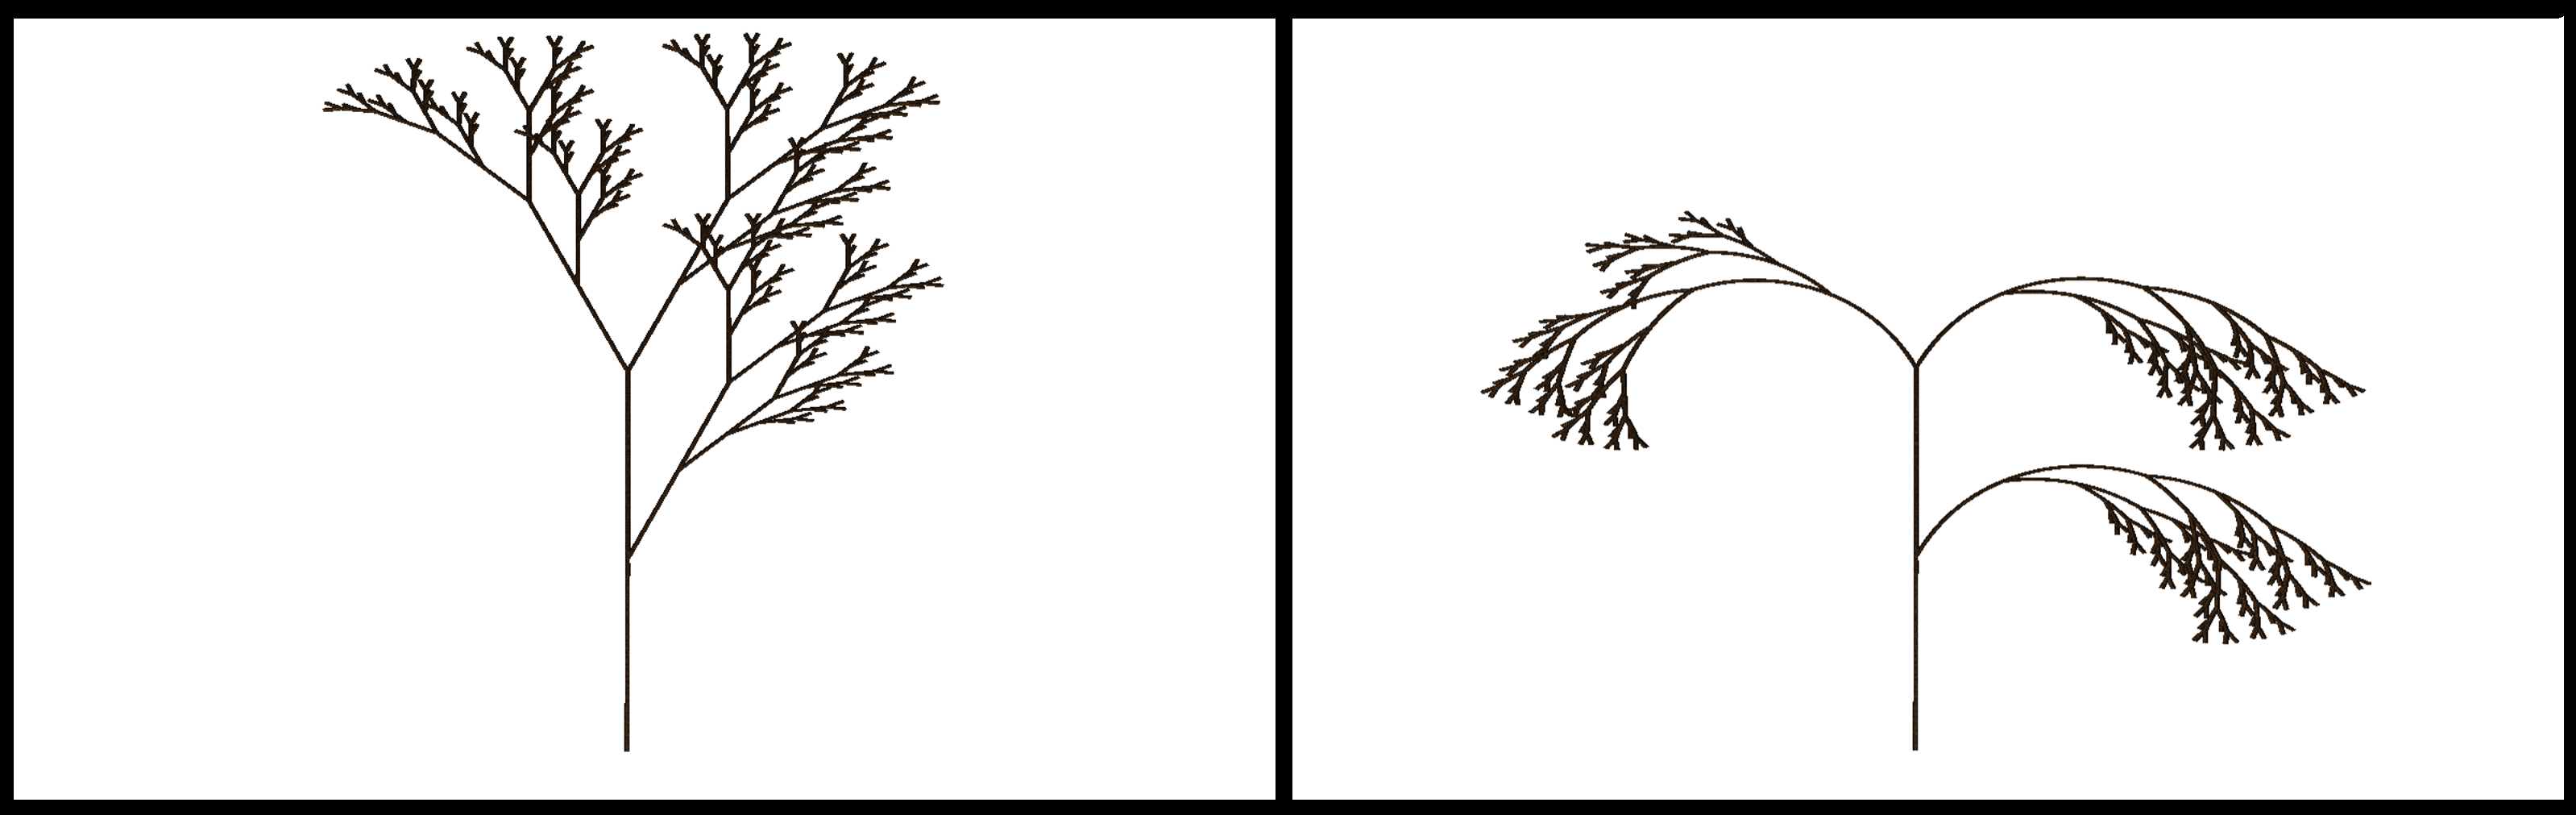
\includegraphics[scale=0.1]{Diagrams/gravityExamples1.png}
		\label{3DAxisFigure} \label{Gravity applied to generated models}
		\caption{Examples simulating gravity on a 2D model}
	}
\end{figure}
\FloatBarrier

The L-system above is a 2D fractal tree that has rendered in three dimensions. It is a 2D tree as it only consists of left and right yaw rotations signified with the `+ and -' symbols without any pitch or roll rotations. In this tree, the rotation `r' is defined as 20$^{\circ}$, the distance `d' is 0.4, and the width `w' is 0.5. The spring constant of the branches is kept at a constant 30.0. This means that all the branches are equally prone to bending. 

\begin{singlespace}
\begin{equation}
\begin{aligned}
	&\textrm{\#n = 5;} \\
	&\textrm{\#object F BRANCH; \#object X SPHERE;}\\
	&\textrm{\#define r 25.7; \#define d 0.5; \#define w 1;}\\
	&\textrm{\#w : !(1.707)X;}\\
	&\textrm{\#p1 : X : * : F(d)[!(w)/(r)+(r)X][!(w)-(r)X][!(w)$\land$(r)X][!(w)\&(r)X]!(w)F(d)X;}\\
	&\textrm{\#p2 : F(s) : * : F(s)F(s);}
\end{aligned}
\end{equation}
\end{singlespace}

\begin{figure}[htbp]
	{\centering
		\vspace{7px}
		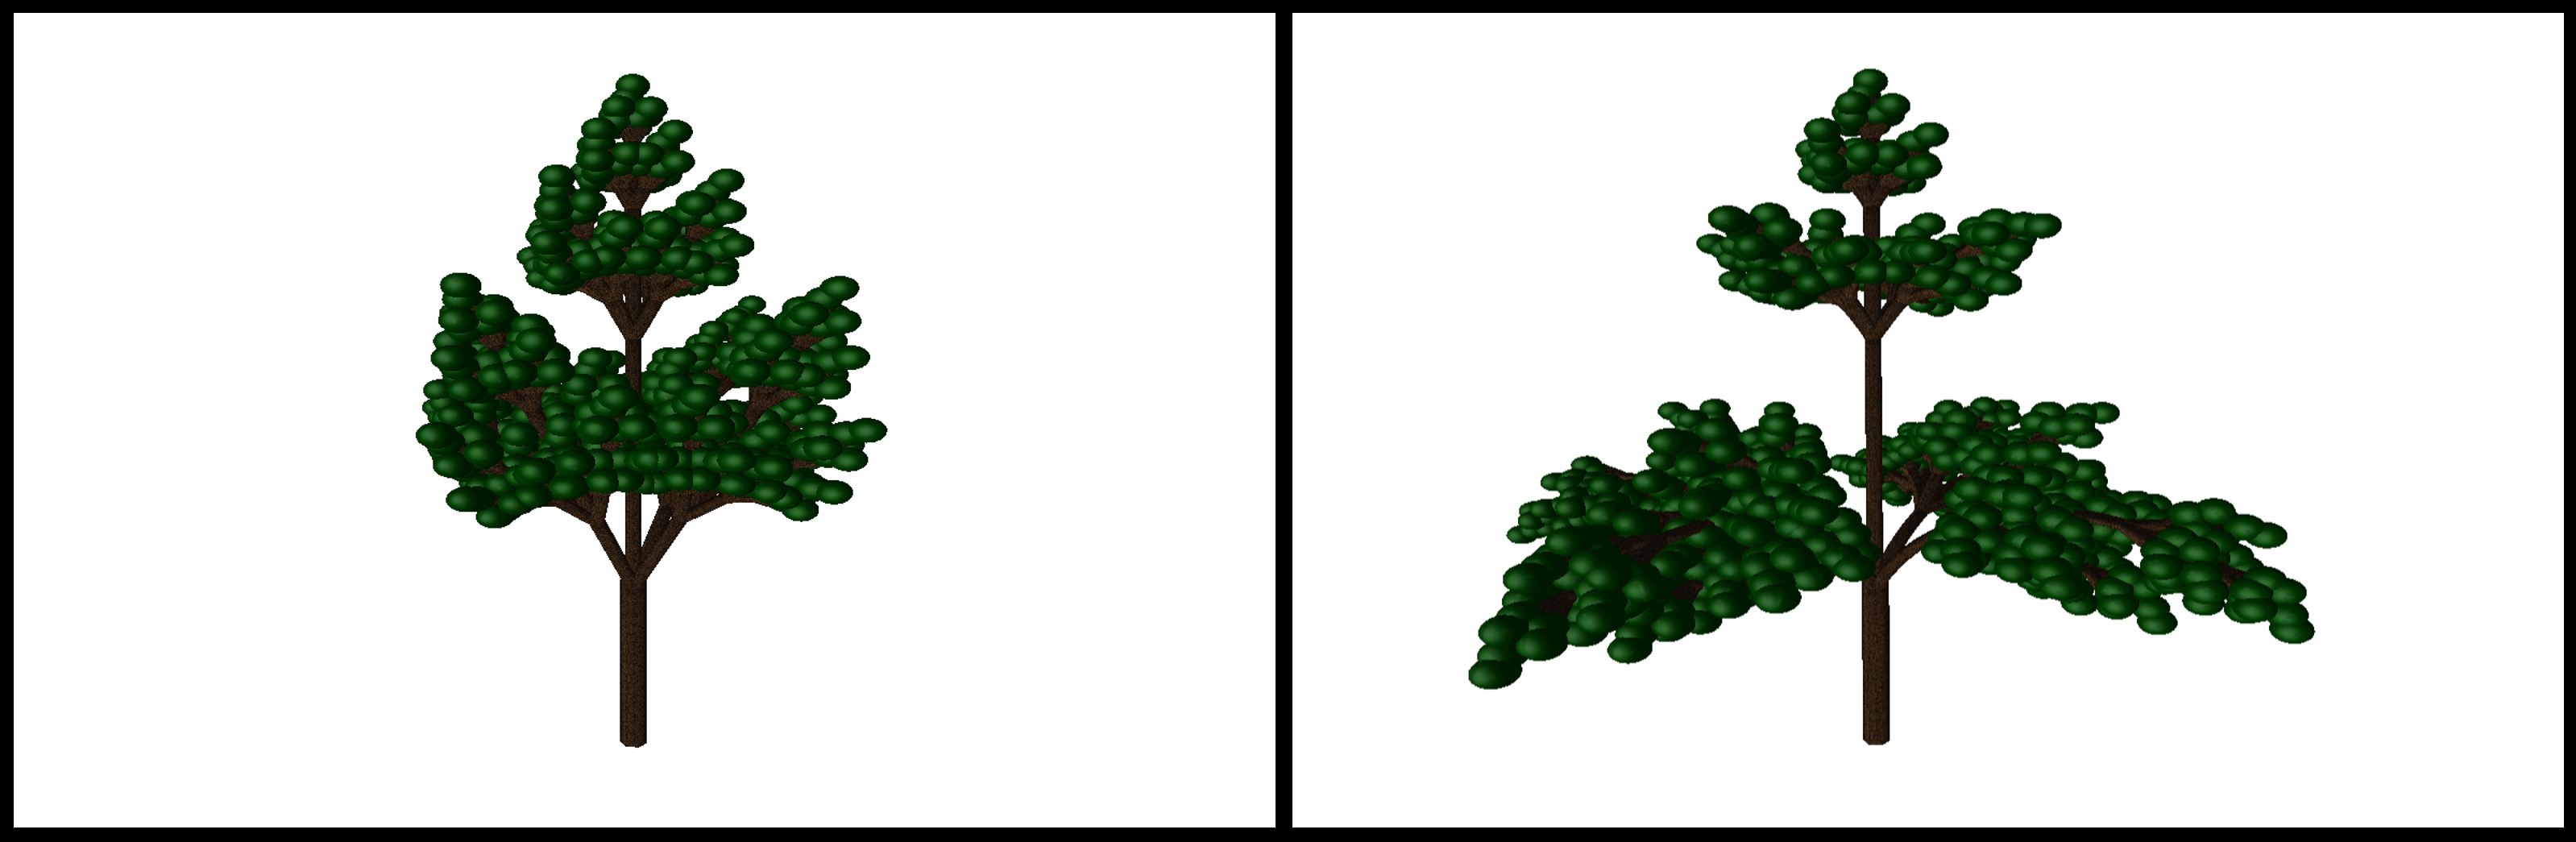
\includegraphics[scale=0.1]{Diagrams/gravityExamples2.png}
		\label{3DAxisFigure} \label{Gravity applied to generated models}
		\caption{Examples simulating gravity on a 3D model}
	}
\end{figure}
\FloatBarrier

\begin{singlespace}
\begin{equation}
\begin{aligned}
	&\textrm{\#n = 6;} \\
	&\textrm{\#object F BRANCH; \#object X SPHERE;}\\
	&\textrm{\#define d1 112.5; \#define d2 157.5; \#define a 22.5;}\\
	&\textrm{\#define lr 1.1; \#define vr 1.4;}\\
	&\textrm{\#w : !(1.4)F(2.0)/(45)A;}\\
	&\textrm{\#p1 : A : * : !(vr)F(2)[\&(a)F(2)AS(1)!(vr)]/(d1)[\&(a)F(2)A S(1)!(vr)]/(d2)[\&(a)F(2)A S(1)!(vr);}\\
	&\textrm{\#p2 : F(l) : * : F(l*lr);}\\
	&\textrm{\#p3 : !(w) : * : !(w*vr);}
\end{aligned}
\end{equation}
\end{singlespace}

\begin{figure}[htbp]
	{\centering
		\vspace{7px}
		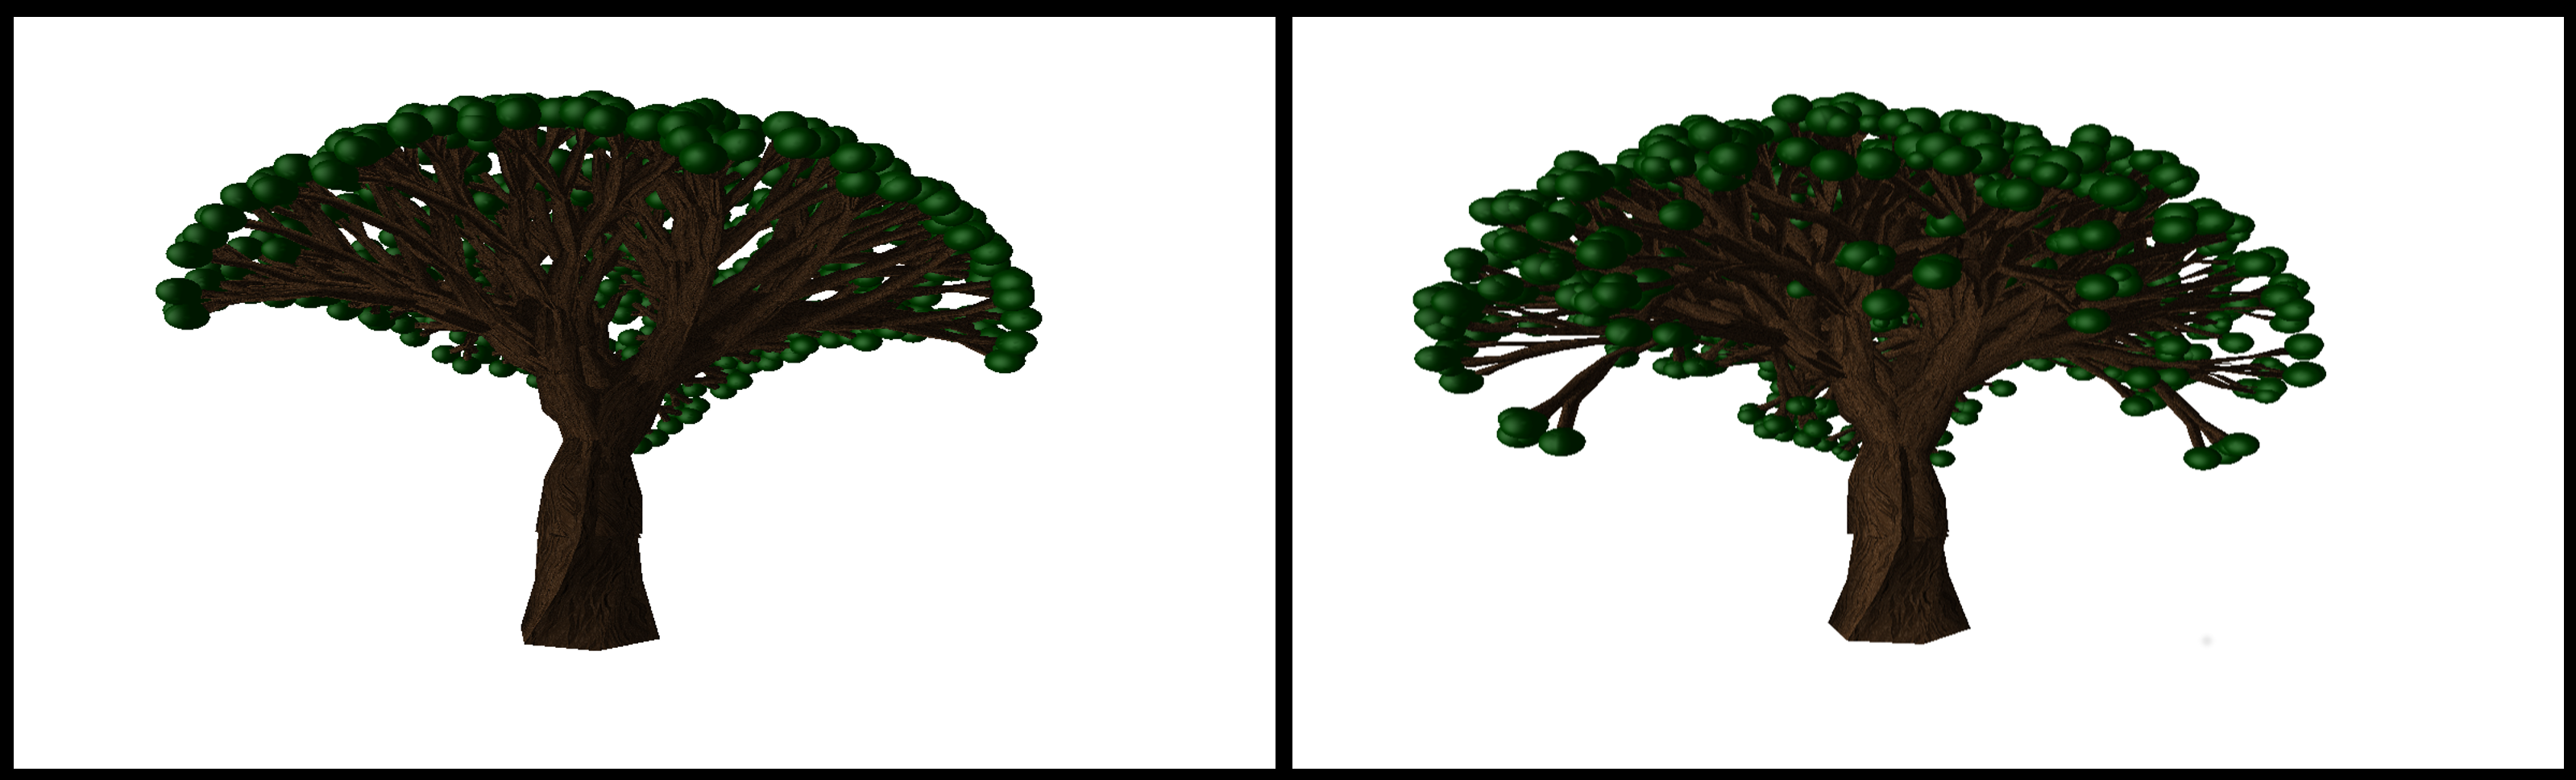
\includegraphics[scale=0.1]{Diagrams/gravityExamples3.png}
		\label{3DAxisFigure} \label{Gravity applied to generated models}
		\caption{Examples simulating gravity on a complex 3D model}
	}
\end{figure}
\FloatBarrier